\chapter{Results}
\label{cha:results}
In this chapter will be illustrated the results obtained in the various texts carried out on the system. Firstly, the performance of the classifier will be explained, and secondly \dots

\section{Classification performance}
The first method experimented to implement the classifier was a data driven approach. 

The dataset taken from \cite{dickinson2015identifying} was filtered, keeping only tweets about a wedding or a birth of a child. Then it was splitted in two files, one for each life event, and every tweet was enriched with Wikipedia entities and topics using the external semantic analyzer. In the end, the wedding dataset counted $2538$ samples, the births one $2233$. Each of these sets were very balance, with half of the sample related to the life event and the other half not. According to the literature, a naive bayes classifier and a decision tree were chosen as classifiers, but due to the better performance of the first one, the second one was initially discarded. In particular, the classifier was a Multinomial Naive Bayes\footnote{\url{http://scikit-learn.org/stable/modules/naive_bayes.html#multinomial-naive-bayes}} available in the \texttt{scikit-learn}\footnote{\url{http://scikit-learn.org/}} library \cite{scikit-learn}.

The very first feature extraction technique was inspired by the \texttt{tf-idf} weight function\footnote{\url{https://it.wikipedia.org/wiki/Tf-idf}}, which is used to undestrand the importance of a word into a series of documents. The idea was to select a small sample of key entities analyzing some web pages focused on the life event taken into consideration, such as a wedding planner homepage or a pregnancy blog. These $k$ top entities were used as features of tweets, and a matrix $X$ was created, with a number of rows equals to the number of tweets and $k$ columns. Each element [$i,j$] of $X$ was a counter of how many times the entity (or topic) $j$ was found in the tweet $i$. However, this methodology performed worse than a random classifier, with both precision and recall scores lower than $0.5$, with $k = 3, 4, 5, 10, 100$.

\begin{table}[htbp]
\centering
\subtable[Results on a single dataset split\label{tab:singlesplit}]{%
\begin{tabular}{cccc}
\hline
Life event & Precision & Recall & F1 Score \\
\hline
\textbf{Getting married} & $0.82$ & $0.81$ & $0.81$ \\
\textbf{Having children} & $0.77$ & $0.78$ & $0.77$ \\
\hline
\end{tabular}
}\qquad\qquad
\subtable[Results on a 10 fold cross validation\label{tab:kfold}]{%
\begin{tabular}{cccc}
\hline
Life event & Precision & Recall & F1 Score \\
\hline
\textbf{Getting married} & $0.73$ & $0.82$ & $0.77$ \\
\textbf{Having children} & $0.62$ & $0.57$ & $0.59$ \\
\hline
\end{tabular}
}
\caption{The performance of the naive bayes were satisfactory on a very balanced dataset. Unfortunatly, users' timelines are very unbalanced, and this classifier turned out to be inappropriate.}
\end{table}

A much better performance with the dataset, but unfortunately not with the reality, was given by using all the Wikipedia entities of the training set as features. Firstly, the dataset was splitted into a training and a test set, the first one with the 70\% of the samples and the second with the remaining 30\%; secondly, a matrix $X$ was created in the same way of the previous attempt, with the difference that this time the number of columns was in the order of thousands. On the test set this solution had good results, as shown in tables~\ref{tab:singlesplit} and \ref{tab:kfold}, but in the reality, trying to predict if tweets from a user timeline were about or not a life event, this solution turned out to be impractical: the discrimination was too loose, and many tweets that wasn't related with the life event at all were considered "positives", with the precision measure that fell dramatically under $0.1$. The overfitting reason was excluded, because the training set was kept aside from everything else. In addition, each sample in the dataset was written by a unique user. The most probable reason is that the dataset used for the training was too balanced compared to the real situation in social networks: in fact, while the dataset contained about 50\% of tweets about a life event and 50\% not, a timeline had a very small percentage of contents about a life event. For example, analyzing a portion of Gareth Bale's Twitter profile\footnote{\url{https://twitter.com/GarethBale11}}, it turned out that on 224 tweets only 2 were about the birth of a child and only one about marriage. Many other profiles considered had similar proportions. 

A third approach was tried, with the purpose of improve the previous situation: train the classifier with a very unbalanced dataset, discarding randomly many of the positive samples to create a 90\% negatives and 10\% positives situation. In each test the positive subset were different, because of randomness, but as before the results were good only with the test set: with a real profile the discrimination was too strong this time, not finding any tweet at all, maybe just because of this disproportion, where too few related samples were given and so the classifier didn't see enough entities among those of positive samples.

Another very big issue was caused by the external semantic analyzer - Dandelion - used to discover Wikipedia entities inside texts. Its results turned out to be very inaccurate for such short texts written in Twitter: for example, a tweet published by a famous sports man about his wedding, with the text "\textit{This is her, my wife}"\footnote{\url{https://twitter.com/petosagan/status/667069250268479488}} was mapped by the analyzer to a song by the British rock band \textit{the Who} called \textit{My Wife}, not undestanding the context at all. Some other cases of misunderstanding between the text and its true meaning were found, for example the word \textit{congratulations} was mapped into the entity "\texttt{Congratulations: 50 Years of the Eurovision Song Contest}", but this was not a big issue because this combination was always respected every time that word was found. Just to be sure that some words were recognized correctly, 4 keywords for each event were manually mapped into their correct entities, such as \textit{baby} on the entity \texttt{Infant}.

\begin{sidewaysfigure}
\centering
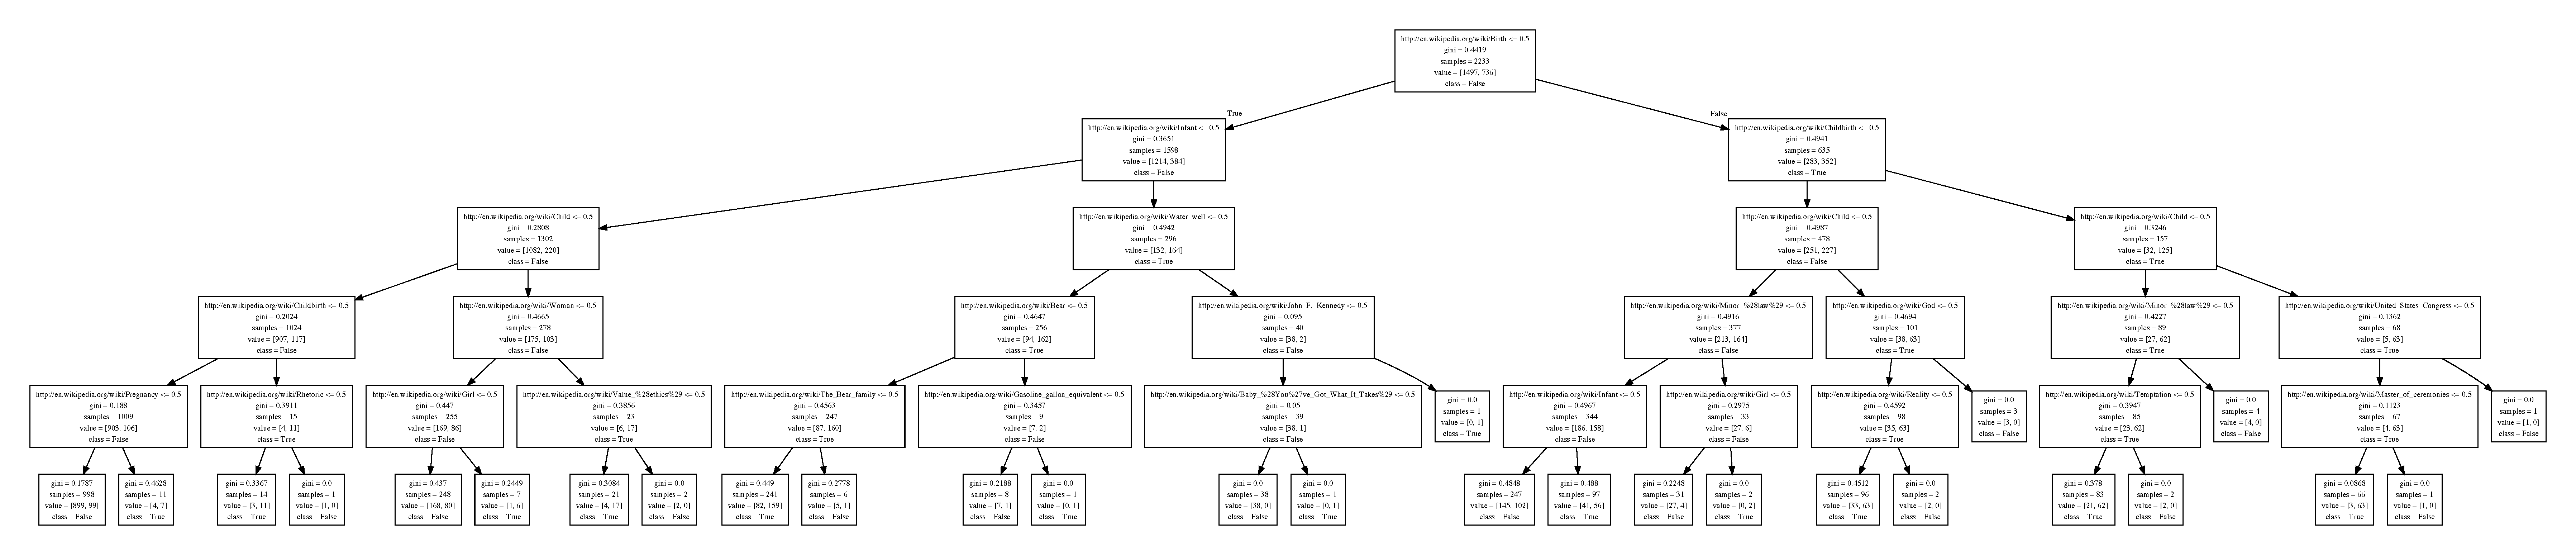
\includegraphics[width=%
1\textwidth]{img/decisiontree}
\caption{The decision tree for the birth of a child event. As can be seen, the nearest nodes to the root are decisions about entities that are strickly connected with the life event itself, and each of them makes a significant split in terms of the size of the resulting subsets, while the deepest nodes are strongly connected with the training set. For this reason the maximum depth was forced to be low.}
\label{fig:decisiontree}
\end{sidewaysfigure}

To avoid issues with the semantic analyzer as much as possible, as few as possible entities were used to classify a tweet: a very first approach consisted in a manual selection of features, for example the entity \texttt{Wife} for wedding, but the results were not satisfactory. The ultimate approach was to let the data decide which entities to use, relying on the dataset taken from \cite{dickinson2015identifying}. The classifier was changed, opting for a decision tree, because the previous naive bayes was too loose during the classification. A decision tree is a machine learning model used for regression and classification based on a binary tree data structure. Each node of the tree is a question relative to a feature of the objects to classifiy, and each leaf represent a decision, an estimation of the value of the input object. During the training, the tree is build starting from the root: at each step of the construction, the goal is to split the dataset into two, making a question on a feature of the objects, to reduce the unpredictability of the two new subsets as much as possible. Every object in input will have its path from the root to a single leaf, which will represent the decision. Precisely, the classifier was the decision tree offered by the \texttt{scikit-learn} library\footnote{\url{http://scikit-learn.org/stable/modules/generated/sklearn.tree.DecisionTreeClassifier.html}}. To reduce the overfitting on the training data, the maximum depth of the tree was limited to 5, so for each root-leaf path, at most 4 intermediate nodes could be found. The decision tree for the life event \texttt{Having Children} can be seen in figure~\ref{fig:decisiontree}. The results with the dataset of \cite{dickinson2015identifying} were a little worse than those of the bayesian classifier shown in tables~\ref{tab:singlesplit} and \ref{tab:kfold}, but in the reality, with a test conducted on 5836 tweets taken by 43 different timelines the results were much better than the previous one, as explained in tables~\ref{tab:treewedding} and \ref{tab:treechild}.

\begin{table}[htbp]
\centering
\subtable[Results about wedding tweets\label{tab:treewedding}]{%
\begin{tabular}{ccccc}
\hline
Sample & Precision & Recall & F1 Score & Support \\
\hline
\textbf{True} & $0.87$ & $0.70$ & $0.77$ & $134$ \\
\textbf{False} & $0.91$ & $0.97$ & $0.94$ & $5702$ \\
\textbf{Avg / Total} & $0.90$ & $0.90$ & $0.90$ & $5836$ \\
\hline
\end{tabular}
}\qquad\qquad
\subtable[Results about birth of a child tweets\label{tab:treechild}]{%
\begin{tabular}{ccccc}
\hline
Sample & Precision & Recall & F1 Score & Support \\
\hline
\textbf{True} & $0.65$ & $0.62$ & $0.63$ & $161$ \\
\textbf{False} & $0.93$ & $0.94$ & $0.94$ & $5675$ \\
\textbf{Avg / Total} & $0.89$ & $0.89$ & $0.89$ & $5836$ \\
\hline
\end{tabular}
}
\caption{The performance of the decision tree with a very unbalanced dataset. On this same test set the previous classifier, the naive bayes, showed both precision and recall scores under 0.1.}
\end{table}